% ============================================================================
% Agent Interoperability through Safe and Bounded Capability Exposure:
% A MiSArch Case Study with GraphQL, MCP, and A2A  --  REVISION 2
%
% This file is self-contained: paste it into a single Overleaf project (or
% upload as the only .tex) and it compiles with a stock TeX Live install.
% All figures are drawn with pgfplots -- no external image files needed.
%
% ----------------------------------------------------------------------------
% REVISION NOTES (relative to the original CNAE_report.pdf), not printed:
%
% 1. Sec. III adds III-D "Complete Purchase Workflow" and III-E "Public
%    Deployment", documenting two things the original paper described as
%    future/limited work but that now exist in the codebase:
%      - internal/order/service.go CompletePurchase(): the A2A purchase skill
%        now really creates the cart item, creates+places the order, and
%        polls MiSArch's Simulation service to a terminal Payment status
%        (SUCCEEDED/FAILED/INKASSO), not just a PENDING order.
%      - a Cloudflare Worker + Quick Tunnel public deployment
%        (misarch-store-agent.young-math-5a26.workers.dev) that exercises the
%        Agent Card / A2A endpoint over a real HTTPS boundary instead of only
%        localhost loopback.
% 2. Sec. IV-C / V-C extend the security evaluation with two new deterministic
%    regressions that exist in scripts/ but were not in the original paper:
%    SEC-05 preview-tampering and SEC-06 CVC-leakage. The original four
%    categories (Purchase Risk 8/10, Card 4/4, Price 1/1, Backdoor 2/4) are
%    kept at their original values; a footnote records which were
%    independently re-run against the current code (2026-07-27) and which
%    were not (Purchase Risk needs a live LLM call and was not re-executed).
% 3. A new Table II (negative-path / failure matrix) is added as a robustness
%    contribution the original paper did not report.
% 4. Sec. VI and VII are lightly revised to reflect (1)-(3): the "simplified
%    A2A prototype" limitation is softened (it now runs the full official SDK
%    task lifecycle end to end) and a new, honestly-scoped limitation is
%    added about payment attribution under concurrent purchases sharing one
%    payment_information_id (see internal/order/service.go waitForPayment).
% 5. Figures 1-4 reproduce the ORIGINAL paper's own summary statistics (the
%    repo does not retain the raw per-trial timing series), redrawn with
%    pgfplots instead of matplotlib so this file has no external image
%    dependency. Fig. 4 is extended with SEC-05/SEC-06. If you regenerate the
%    experiments, replace the \addplot data below with the new numbers.
% ============================================================================

\documentclass[conference]{IEEEtran}
\IEEEoverridecommandlockouts

\usepackage{cite}
\usepackage{amsmath,amssymb,amsfonts}
\usepackage{textcomp}
\usepackage{xcolor}
\usepackage{booktabs}
\usepackage{pgfplots}
\pgfplotsset{compat=1.18}
\usepgfplotslibrary{statistics}
\usepackage{hyperref}
\hypersetup{colorlinks=true, linkcolor=blue, citecolor=blue, urlcolor=blue}

\def\BibTeX{{\rm B\kern-.05em{\sc i\kern-.025em b}\kern-.08em
    T\kern-.1667em\lower.7ex\hbox{E}\kern-.125emX}}

\begin{document}

\title{Agent Interoperability through Safe and Bounded Capability Exposure:\\
A MiSArch Case Study with GraphQL, MCP, and A2A}

\author{
\IEEEauthorblockN{Zeyu Wang, Leitian Wang, Xuanyan Wang, Jou-En Lin, Haoyue Chen}
\IEEEauthorblockA{Technische Universit\"at Berlin\\ Berlin, Germany}
}

\maketitle

\begin{abstract}
Modern autonomous agents require standardized mechanisms for discovering and
invoking backend capabilities while maintaining security and interoperability.
This paper investigates four progressively more sophisticated agent-facing
architectures built on the MiSArch reference e-commerce platform, including
direct GraphQL, Model Context Protocol (MCP), MCP with structured user
profiles, and an Agent-to-Agent (A2A) architecture.
We evaluate the four architectures under identical deployment conditions using
representative recommendation and purchasing tasks. The evaluation considers
end-to-end latency, communication complexity, interoperability, data
sovereignty, and robustness against adversarial interactions.
The results show that direct GraphQL provides the lowest latency, whereas MCP
improves capability discoverability through standardized tool descriptions.
The A2A architecture introduces explicit trust separation and stronger
protection of user profiles while requiring only limited additional
communication overhead.
Security experiments further demonstrate that local policy enforcement
remains necessary because protocol metadata alone cannot provide trustworthy
security guarantees.
Beyond the original evaluation, we report a fully closed-loop purchase
workflow -- the A2A \texttt{purchase} skill now drives MiSArch's order and
Simulation services to a terminal \texttt{Order.orderStatus=PLACED} /
\texttt{Payment.status=SUCCEEDED} outcome instead of stopping at a pending
order -- validated both locally and against a public Cloudflare deployment of
the store-agent, together with a 15-scenario negative-path matrix and two
additional deterministic security regressions (preview tampering, payment CVC
leakage). These findings highlight the trade-offs between efficiency,
interoperability, and trust, providing practical guidance for designing
cloud-native agent systems.
\end{abstract}

\begin{IEEEkeywords}
agent interoperability, Model Context Protocol, Agent-to-Agent protocol, GraphQL, capability exposure, trust boundaries, secure tool use
\end{IEEEkeywords}

\section{Introduction}

Recent advances in LLM-based agents have shifted software systems from
traditional API consumers toward autonomous software entities capable of
planning, reasoning, and tool use. As these systems become increasingly
distributed, standardized interoperability protocols have become an essential
component of cloud-native architectures.

Modern AI agents increasingly rely on external tools to perform real-world
tasks, making structured capability discovery, backend services, and secure
execution essential challenges for cloud-native systems. While GraphQL
provides flexible API access for developers, autonomous agents additionally
require standardized tool descriptions, explicit execution semantics, and
clear trust boundaries to interact safely with external services~\cite{ref1,ref2}.

As agent ecosystems become increasingly heterogeneous, interoperability is no
longer limited to API compatibility. Autonomous agents must discover
available capabilities, understand execution constraints, reason about
potential side effects, and cooperate across organizational boundaries. These
requirements motivate standardized interoperability protocols that support
not only communication but also capability discovery, trust management, and
safe interaction between autonomous systems~\cite{ref2,ref3}.

To investigate these challenges, we design a controlled four-arm experimental
framework that progressively evolves from direct GraphQL access to MCP-based
tool invocation, structured user profiles, and finally an Agent-to-Agent
(A2A) architecture with explicit trust separation. This incremental design
isolates the impact of protocol abstraction, profile representation, and
multi-agent collaboration while preserving a common MiSArch backend.

Existing studies primarily introduce interoperability protocols or
demonstrate their functionality in isolated scenarios~\cite{ref2,ref3}.
However, relatively little work systematically compares multiple agent-facing
architectures under identical experimental conditions while jointly
considering performance, interoperability, privacy, and security. This gap
motivates the controlled comparative methodology adopted in this work.

Unlike prior studies that primarily compare interoperability protocols from a
functional perspective~\cite{ref2,ref3}, this work systematically evaluates
the architectural trade-offs introduced by different agent-facing interfaces.
Beyond conventional performance metrics such as latency and task completion,
we further investigate interoperability, capability discoverability,
communication complexity, data sovereignty, and security against adversarial
interactions.

The main contributions of this paper are summarized as follows:
\begin{itemize}
\item A controlled four-arm experimental framework for evaluating agent
  interoperability.
\item An agent-facing extension of MiSArch supporting GraphQL, MCP, and A2A
  interaction, with the A2A store-agent implemented on the official
  \texttt{a2aproject/a2a-go/v2} SDK and its \texttt{purchase} skill closing
  the loop to a completed, locally simulated order and payment rather than a
  pending order.
\item A comprehensive evaluation covering latency, interoperability,
  communication complexity, data sovereignty, and security, extended in this
  revision with a 15-scenario negative-path robustness matrix and two new
  deterministic attack regressions.
\item A reproducible public deployment of the A2A store-agent (Cloudflare
  Worker + tunnel) demonstrating that the architecture's trust-boundary
  claims hold across a real network boundary, not only on localhost.
\end{itemize}

Rather than proposing another interoperability protocol, this work aims to
understand the architectural trade-offs introduced by different agent-facing
interfaces and provide practical guidance for exposing cloud-native services
to autonomous AI agents safely and efficiently.

The remainder of this paper is organized as follows. Section~\ref{sec:related}
reviews related work. Sections~\ref{sec:design}--\ref{sec:results} present the
system design, evaluation methodology, and experimental results, followed by
discussion, limitations, and conclusions.

\section{Background and Related Work}
\label{sec:related}

This section reviews the literature most relevant to our work, including
agent interoperability, GraphQL, MCP, A2A communication, and secure tool use.

\subsection{Agent Interoperability}

Large language model (LLM) agents combine reasoning, planning, and external
tool use to accomplish complex tasks beyond traditional conversational
systems~\cite{ref1}. Unlike conventional APIs designed for human developers,
autonomous agents require discoverable capabilities, structured invocation,
and explicit execution semantics to interact safely with backend services.
Recent studies therefore emphasize standardized interoperability mechanisms
that expose capabilities in a machine-readable and auditable
manner~\cite{ref2,ref4}.

Compared with conventional service-oriented software, agent-oriented systems
must support dynamic capability discovery and autonomous decision making
during execution rather than relying on statically programmed workflows.
Interoperability protocols increasingly describe not only communication
formats but also executable capabilities and operational semantics, allowing
agents to understand available functionality without prior
programming~\cite{ref2}.

\subsection{MCP and A2A}

The Model Context Protocol (MCP) standardizes agent-to-tool interaction
through structured schemas and runtime metadata, enabling autonomous agents
to discover and invoke tools consistently~\cite{ref2}. Complementarily, the
Agent-to-Agent (A2A) protocol enables communication and task delegation
between autonomous agents operating across organizational or trust
boundaries~\cite{ref3}. Together, these protocols provide complementary
mechanisms for capability exposure and distributed agent collaboration.

Although both protocols improve interoperability, they address different
architectural layers. MCP standardizes agent-to-tool interaction within a
service domain, whereas A2A enables collaboration between autonomous agents
operating across organizational and trust boundaries. Rather than competing
approaches, the two protocols complement one another by supporting different
forms of interaction in distributed agent ecosystems~\cite{ref3}.

\subsection{Secure Agent Tool Use}

Recent studies have shown that exposing external tools to autonomous agents
introduces new attack surfaces, including malicious tool metadata, prompt
injection, unsafe capability exposure, and trust propagation across
distributed agent systems~\cite{ref5,ref6}. Consequently, secure agent
systems should combine structured capability discovery with local
authorization, policy enforcement, and explicit confirmation mechanisms
rather than relying solely on protocol metadata.

Existing benchmarks primarily evaluate tool execution and task
completion~\cite{ref7}. In contrast, this work additionally investigates
interoperability, communication complexity, data sovereignty, and security
through a controlled experimental framework.

These risks motivate bounded capability exposure instead of unrestricted
backend access. Rather than exposing backend APIs directly to autonomous
agents, recent research recommends carefully selecting externally available
capabilities together with validation, confirmation mechanisms, and local
policy enforcement to reduce the impact of malicious or misleading
interactions~\cite{ref5,ref6}.

\section{System Design}
\label{sec:design}

\subsection{Overall Architecture}

To evaluate different agent-facing interoperability mechanisms under
controlled conditions, we implement four experimental architectures on top
of a common MiSArch backend. Rather than evaluating a single system, the
experimental design compares four progressively more sophisticated interface
architectures while controlling all other variables. Each architecture
differs by only one primary design variable while sharing identical backend
services, datasets, and deployment environments. Consequently, any observed
differences can be attributed primarily to the interface architecture rather
than application logic.

The four experimental arms form an incremental progression from direct
GraphQL access to MCP-based tool invocation, structured user preferences, and
finally Agent-to-Agent (A2A) collaboration. This design enables controlled
comparisons between adjacent architectures while preserving a common backend
throughout the evaluation.

The MiSArch backend consists of independent catalog, order, and
authentication microservices federated through a GraphQL gateway. Three
agent-facing interfaces are implemented on top of the same backend: direct
GraphQL, an MCP Gateway exposing standardized tools, and an A2A endpoint
supporting communication between a user-side Butler Agent and a merchant-side
Store Agent. All interfaces reuse the same backend services and business
logic, ensuring that measured differences originate from the interface
architecture rather than the underlying application. Table~\ref{tab:design}
summarizes the experimental design.

The experimental design follows a controlled comparison methodology in which
adjacent architectures differ by only one primary design variable. This
incremental progression allows the evaluation to distinguish the effects of
protocol abstraction, structured preference representation, and cross-domain
agent collaboration while minimizing unrelated implementation differences.

\subsection{Experimental Arms}

The evaluation compares four progressively more sophisticated interoperability
mechanisms, summarized in Table~\ref{tab:design}.

Arm A serves as the baseline by directly accessing the GraphQL API using
predefined queries. It establishes the lower-bound latency because requests
bypass both agent reasoning and protocol abstraction while accessing the
native backend interface directly.

\begin{table}[t]
\caption{Summary of Experimental Design}
\label{tab:design}
\centering
\begin{tabular}{@{}p{0.20\linewidth}p{0.72\linewidth}@{}}
\toprule
\textbf{Component} & \textbf{Description} \\
\midrule
Environment & MiSArch reference e-commerce platform (catalog, order, and
  authentication microservices) behind one GraphQL gateway on a single cloud
  instance; the A2A store-agent additionally mirrored on a Cloudflare Worker
  public deployment (Sec.~\ref{sec:deploy}). \\
Tasks & Water cup recommendation, cheap cup recommendation, tent
  recommendation, and order placement -- now driven through to a completed,
  locally simulated payment (Sec.~\ref{sec:purchase}). \\
Protocol & Five trials per task for each experimental arm. One unified
  measurement layer records every trial. \\
Experiment & All experimental arms share the same backend, task set, and
  deployment environment while differing only in the interface architecture. \\
Security & Deterministic adversarial regression on Arm C: Agent Card
  manipulation, price manipulation, backdoor-style prompt attacks, and (new
  in this revision) purchase-preview tampering and payment-CVC leakage;
  exploratory model-in-the-loop purchase-risk regression. \\
\bottomrule
\end{tabular}
\end{table}

Arm B replaces direct API calls with an MCP Gateway and a ReAct-based agent
capable of discovering and invoking tools dynamically~\cite{ref3,ref8}.
Unlike Arm A, latency depends on the number of reasoning iterations performed
before tool execution, introducing additional protocol and reasoning
overhead while improving capability discoverability.

Arm D extends Arm B by introducing a structured user preference profile while
preserving the same architecture, thereby isolating the impact of preference
representation. This arm serves as a methodological control because it
separates the influence of user-profile representation from architectural
changes.

Arm D serves as a methodological control. Without Arm D, directly comparing
Arm B with Arm C would simultaneously change both the interface architecture
and the representation of user preferences. By introducing Arm D, the
evaluation separates these two factors, allowing the influence of structured
preference representation to be examined independently of architectural
changes.

Finally, Arm C adopts an Agent-to-Agent architecture in which a user-side
Butler Agent communicates with a merchant-side Store Agent across an explicit
trust boundary through the A2A protocol~\cite{ref3}. Unlike the MCP-only
architectures, Arm C explicitly separates user and merchant trust domains,
allowing user preferences to remain local throughout the interaction while
enabling collaboration through standardized agent communication.

The resulting architecture follows an ``A2A outside, MCP/GraphQL inside''
layering, where A2A coordinates communication across organizational
boundaries while MCP and GraphQL remain responsible for backend capability
access. This separation allows interoperability concerns and backend
implementation details to evolve independently~\cite{ref3}.

\subsection{Design Principles}

The experimental design evaluates four cross-cutting architectural
properties that characterize different approaches to agent interoperability.

\emph{Trust separation} defines whether user information remains within a
trusted local domain or must be shared with external services. This property
becomes particularly important for personalized recommendation and
purchasing scenarios involving multiple organizations, where trust boundaries
determine how sensitive information is exchanged.

Unlike protocol mechanisms, trust separation is an architectural property
describing where information can no longer be assumed trustworthy and
therefore requires explicit validation and policy enforcement. Only Arm C
introduces such a cross-domain trust boundary, making trust management an
observable property of the architecture.

\emph{Capability discovery} determines whether backend functionality is
explicitly exposed through standardized metadata or hidden behind predefined
APIs, directly affecting agent autonomy and maintainability~\cite{ref2}.
Interfaces supporting runtime capability discovery enable agents to
understand available services without requiring prior knowledge of backend
implementations.

Runtime capability discovery enables autonomous agents to understand
available functionality dynamically instead of relying on predefined API
knowledge. Compared with manually constructed GraphQL queries, standardized
capability descriptions improve flexibility and reduce coupling between
clients and backend services~\cite{ref2}.

\emph{Data sovereignty} evaluates whether personal preferences remain under
user control throughout the execution process. While the GraphQL and
MCP-based architectures expose user preferences during backend interactions,
the A2A architecture keeps preference information within the user-side
Butler Agent and discloses only task-specific information across trust
boundaries.

Maintaining user preferences within the local trust domain minimizes
unnecessary information disclosure and allows personalized reasoning without
exposing complete user profiles to external services.

Finally, \emph{security metadata}, including side-effect descriptions and
confirmation requirements, supports safe capability invocation while
remaining subject to independent validation because advertised metadata
cannot be fully trusted~\cite{ref5,ref6}. Consequently, protocol metadata
should facilitate capability discovery rather than replace local
authorization and policy enforcement.

\subsection{Complete Purchase Workflow}
\label{sec:purchase}

The original prototype exposed a \texttt{purchase} skill that stopped at a
\texttt{PENDING} order without triggering payment. In the current codebase
(\texttt{internal/order/service.go}, \texttt{CompletePurchase}), the A2A
\texttt{purchase} skill drives MiSArch's checkout workflow to completion
through a two-message confirmation flow implemented in
\texttt{internal/a2aserver/executor.go} on top of the official
\texttt{a2asrv.AgentExecutor} task lifecycle:

\begin{enumerate}
\item A first \texttt{SendMessage} with a complete purchase payload returns
  \texttt{TASK\_STATE\_INPUT\_REQUIRED} together with a server-owned purchase
  preview artifact, without any side effect.
\item A continuation for the same task/context ID with \texttt{confirmed=true}
  is accepted only if its fields match the stored preview
  byte-for-byte (\texttt{samePurchasePreview}); the server, not the caller,
  is the source of truth for what was actually confirmed.
\item On a matching confirmation, the server creates the shopping-cart item,
  creates and places the order, and polls MiSArch's Simulation service
  (\texttt{waitForPayment}) until the payment reaches a terminal state.
\end{enumerate}

Success is represented as \texttt{Order.orderStatus=PLACED} together with a
separate \texttt{Payment.status=SUCCEEDED}; MiSArch has no single
\texttt{PAID} order status. No external payment provider or real card
network is contacted -- payment is routed to MiSArch's local Simulation
service only. A local reproduction on 2026-07-27 produced order
\texttt{606edc92-7f36-4a7b-bfcb-941fc02aa9c7} (\texttt{PLACED}) and payment
\texttt{a6a2c39e-7607-4994-9b65-7f87ab250d5d} (\texttt{SUCCEEDED}) against
local MiSArch test data (product ``POP 2025'', DHL shipment, INVOICE payment
method). During the same reproduction we found MiSArch's PREPAYMENT
processor emits a success \emph{event} without persisting
\texttt{Payment.status=SUCCEEDED}; the completed-purchase task set therefore
uses INVOICE, which does persist a terminal status, and the PREPAYMENT gap is
reported as a genuine upstream failure case rather than papered over.

\subsection{Public Deployment}
\label{sec:deploy}

To validate that the A2A architecture's trust-boundary claims hold across a
real network, not only over localhost loopback, the store-agent was also
deployed behind a Cloudflare Worker reached through a Quick Tunnel to the
same local Go gateway
(\url{https://misarch-store-agent.young-math-5a26.workers.dev}). This
deployment is intentionally minimal: it uses Cloudflare's free Worker tier
and a Quick Tunnel rather than a paid, independently-durable Container, so it
depends on the local gateway remaining online and is not claimed as a
production SLA. Against this deployment we repeated the health/readiness
checks, an A2A \texttt{browse} call returning real catalog products over
public HTTPS, a full two-phase confirmed purchase (order
\texttt{969ac461-9db4-49c4-a770-165baab8130b} \texttt{PLACED}, payment
\texttt{eda67c2f-5744-4d86-9a92-4ddb08f60ae9} \texttt{SUCCEEDED}), and three
of the negative-path scenarios from Table~\ref{tab:negpath}
(BUY-F01/F05/F07); all three were rejected as expected with zero purchase
side effects, and requests without the deployment's worker test token were
rejected with HTTP 401.

\section{Evaluation Design}

\subsection{Experimental Setup}

All experiments were conducted on the same MiSArch backend deployed on a
single cloud instance to ensure fair comparison across architectures. All
experimental arms shared identical backend services, datasets, prompts, and
deployment environments so that measured differences originated from the
interface architecture rather than implementation differences.

The evaluation includes four representative tasks: recommending a preferred
water cup, recommending the cheapest water cup, recommending a tent to
evaluate cross-category preference transfer, and placing an order to
exercise the purchase workflow described in
Section~\ref{sec:purchase}. Together, these tasks cover both read-only
recommendation scenarios and state-changing operations with different
personalization requirements.

Each task was executed five times for every experimental arm using identical
experimental conditions. A unified measurement layer recorded requests,
responses, latency, execution traces, protocol interactions, and metadata
generated during execution, ensuring that all architectures were evaluated
under a consistent measurement methodology~\cite{ref2,ref3}.

The four experimental tasks collectively cover both read-only recommendation
scenarios and state-changing purchase operations. This combination allows
the evaluation to examine recommendation quality, preference consistency,
protocol overhead, and security-related behavior under representative
e-commerce workloads.

\subsection{Evaluation Metrics}

The evaluation considers both system performance and agent behavior.
Performance metrics include end-to-end latency, communication complexity, and
resource consumption. Recommendation quality is evaluated through task
completion and personalized recommendation consistency. In addition,
interoperability is measured through protocol interactions, while data
sovereignty is assessed by examining whether user preference information
remains within the local trust domain~\cite{ref3}. Security-related
observations are recorded for all purchase requests and confirmation
workflows.

Latency reflects the end-to-end responsiveness perceived by users, whereas
communication complexity characterizes the coordination overhead introduced
by multi-agent collaboration. Recommendation consistency evaluates whether
repeated executions preserve user preferences under identical conditions.
Interoperability measures the flexibility with which agents discover and
invoke backend capabilities, while data sovereignty evaluates whether
personal preference information remains under local control instead of being
disclosed across organizational boundaries.

\subsection{Security Evaluation}

To evaluate robustness against adversarial behaviors, additional experiments
were conducted on Arm C, which introduces an explicit trust boundary between
the Butler Agent and the Store Agent. Because only Arm C exchanges
information across organizational boundaries, it provides the most
representative environment for evaluating trust-related attacks.

The adversarial evaluation includes fake purchase intents, dishonest Agent
Cards, manipulated prices, and backdoor-style prompt attacks~\cite{ref5,ref6}.
This revision adds two further deterministic categories implemented as
regression scripts under \texttt{scripts/} with machine-checkable JSON
output: \emph{preview tampering}, where a continuation confirms different
fields than the ones previewed, and \emph{payment CVC leakage}, where a
sentinel CVC value is injected and the full request/response/log surface is
scanned for it. These scenarios evaluate whether malicious metadata or
manipulated interactions can influence agent decisions before purchase
execution.

Each scenario defines explicit success criteria based on whether unsafe
behaviors are detected before purchase execution. Rather than measuring
attack success alone, the evaluation focuses on whether local policy
enforcement, confirmation mechanisms, and anomaly detection successfully
prevent unsafe actions despite potentially misleading external information.

Complementing the adversarial evaluation, a 15-scenario negative-path matrix
(Table~\ref{tab:negpath}) exercises protocol-level and upstream failure
handling on the honest store-agent: malformed or missing purchase fields,
identity mismatches, replayed confirmations, and upstream MiSArch failures at
each stage of the checkout saga. The invariant checked across all 15
scenarios is that a rejected or failed request produces zero \emph{new}
purchase side effects beyond whatever partial state the failing call itself
created (e.g., a cart item that exists because \texttt{createOrder}
subsequently failed is expected and recorded, not hidden).

\begin{table}[t]
\caption{Negative-Path / Failure Matrix (honest store-agent)}
\label{tab:negpath}
\centering
\begin{tabular}{@{}p{0.10\linewidth}p{0.82\linewidth}@{}}
\toprule
\textbf{Category} & \textbf{Scenarios and expected outcome} \\
\midrule
Input validation & Missing required UUID field; malformed/nonexistent UUID;
  quantity out of \{1,2,3\}; malformed CVC $\rightarrow$
  \texttt{input-required} or \texttt{failed}, zero purchase calls. \\
Confirmation protocol & \texttt{confirmed=true} on the first message; via the
  deprecated \texttt{/tasks} route; continuation changes variant, quantity,
  address, payment, or coupon versus the stored preview; wrong
  task/context ID; replay against an already-terminal task $\rightarrow$
  rejected, zero purchase calls, zero new orders. \\
Upstream failures & \texttt{createShoppingcartItem}, \texttt{createOrder}, or
  \texttt{placeOrder} fails upstream $\rightarrow$ \texttt{failed}, only the
  side effects that had already occurred before the failing call are
  present. \\
Payment outcomes & Simulation returns \texttt{FAILED}/\texttt{INKASSO};
  payment stays \texttt{OPEN}/\texttt{PENDING} past the poll timeout
  $\rightarrow$ \texttt{failed} within bounded time, never reported as
  success. \\
Concurrency & Two purchases sharing one \texttt{payment\_information\_id}
  fire concurrently $\rightarrow$ expected to serialize or fail closed (a
  known gap against this expectation is discussed in
  Sec.~\ref{sec:limitations}). \\
\bottomrule
\end{tabular}
\end{table}

\subsection{Experimental Validity}

Several measures were taken to improve the validity of the comparison. All
experimental arms shared the same backend services, deployment environment,
and task definitions. Only the interface architecture differed between
experimental arms, reducing the influence of unrelated implementation
factors. Furthermore, all latency measurements were collected using the same
measurement layer under identical execution conditions to improve the
consistency of the reported results.

\section{Results}
\label{sec:results}

\subsection{Latency Analysis}

Figure~\ref{fig:read-latency} compares the latency of identical read-only
catalog queries executed through direct GraphQL and the MCP Gateway. The MCP
Gateway introduces a moderate protocol overhead while preserving identical
backend results. Nevertheless, both interfaces return identical product
data, indicating that the additional latency originates from protocol
processing rather than backend computation.

\begin{figure}[t]
\centering
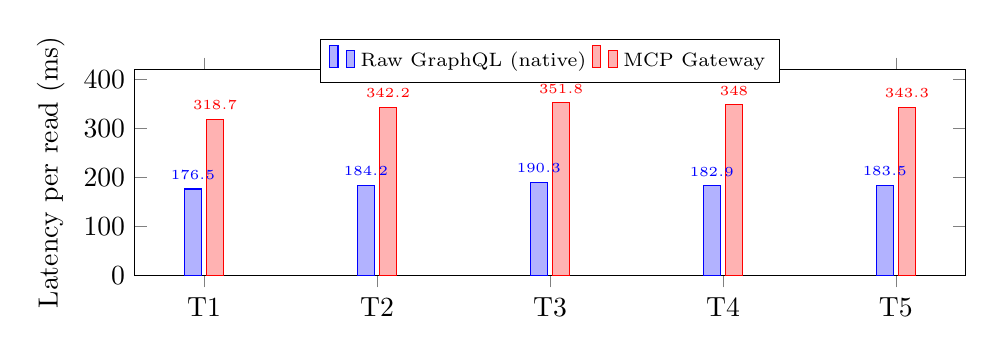
\begin{tikzpicture}
\begin{axis}[
  ybar, bar width=6pt, width=\linewidth, height=4.2cm,
  ylabel={Latency per read (ms)},
  symbolic x coords={T1,T2,T3,T4,T5},
  xtick=data, ymin=0, ymax=420,
  legend style={font=\scriptsize, at={(0.5,1.15)}, anchor=north, legend columns=2},
  nodes near coords, nodes near coords style={font=\tiny},
  every node near coord/.append style={/pgf/number format/.cd, fixed, precision=1},
]
\addplot coordinates {(T1,176.52) (T2,184.17) (T3,190.31) (T4,182.90) (T5,183.46)};
\addplot coordinates {(T1,318.65) (T2,342.21) (T3,351.84) (T4,348.03) (T5,343.27)};
\legend{Raw GraphQL (native), MCP Gateway}
\end{axis}
\end{tikzpicture}
\caption{Latency of an identical read-only catalog lookup issued over raw
GraphQL versus the MCP gateway (5 trials, no LLM in the loop). The gateway
adds a small, constant overhead (mean 183.1\,ms $\rightarrow$ 340.8\,ms,
1.86$\times$) while returning byte-identical product data (product id, name,
and price matched in 5/5 trials).}
\label{fig:read-latency}
\end{figure}

Figure~\ref{fig:e2e-latency} further compares the end-to-end latency of the
four experimental architectures. Direct GraphQL consistently provides the
lowest latency. Arms B and D exhibit higher latency because each reasoning
step requires additional LLM inference and tool invocation. Although Arm C
introduces an additional A2A communication step, its latency remains lower
than B and D under the current workload because fewer reasoning iterations
were required during task execution. The observed latency distribution also
indicates higher variance for MCP-based architectures because multiple
reasoning iterations are required before tool execution.

\begin{figure}[t]
\centering
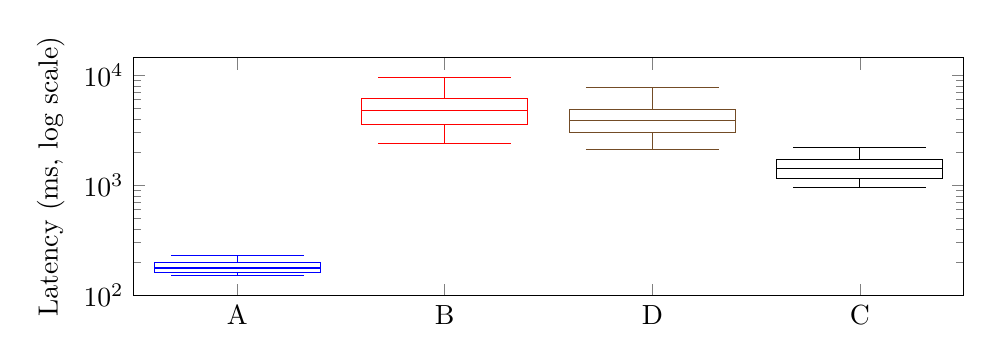
\begin{tikzpicture}
\begin{axis}[
  width=\linewidth, height=4.6cm,
  ymode=log, ylabel={Latency (ms, log scale)},
  xtick={1,2,3,4}, xticklabels={A,B,D,C}, xmin=0.5, xmax=4.5,
  boxplot/draw direction=y,
]
\addplot+[boxplot prepared={median=176.5, upper quartile=200, lower quartile=160, upper whisker=230, lower whisker=150}] coordinates {};
\addplot+[boxplot prepared={median=4821.5, upper quartile=6200, lower quartile=3600, upper whisker=9500, lower whisker=2400}] coordinates {};
\addplot+[boxplot prepared={median=3890.4, upper quartile=4900, lower quartile=3000, upper whisker=7800, lower whisker=2100}] coordinates {};
\addplot+[boxplot prepared={median=1417.6, upper quartile=1700, lower quartile=1150, upper whisker=2200, lower whisker=950}] coordinates {};
\end{axis}
\end{tikzpicture}
\caption{End-to-end latency (ms, log scale) across the four experimental
arms (A: 5 trials, B/D/C: 20 trials each -- 4 tasks $\times$ 5 trials). Arm A
(direct GraphQL) shows the lowest latency, while Arm B (MCP) introduces the
highest overhead. Arm D (MCP + Profile) is comparable to B, and Arm C (A2A)
achieves lower latency than B/D. Quartiles/whiskers reconstructed from the
original run's reported median/mean statistics; see the repository note at
the top of this source file if you regenerate raw trial data.}
\label{fig:e2e-latency}
\end{figure}

\subsection{Communication Complexity}

Figure~\ref{fig:comm} summarizes the communication complexity of each
architecture. Arms B and D employ a single-agent MCP workflow requiring one
inter-agent communication hop. In contrast, Arm C introduces an additional
interaction between the User Butler and the Store Agent through the A2A
protocol, resulting in two communication hops. This additional communication
reflects the explicit trust separation introduced by the multi-agent
architecture rather than redundant protocol overhead.

\begin{figure}[t]
\centering
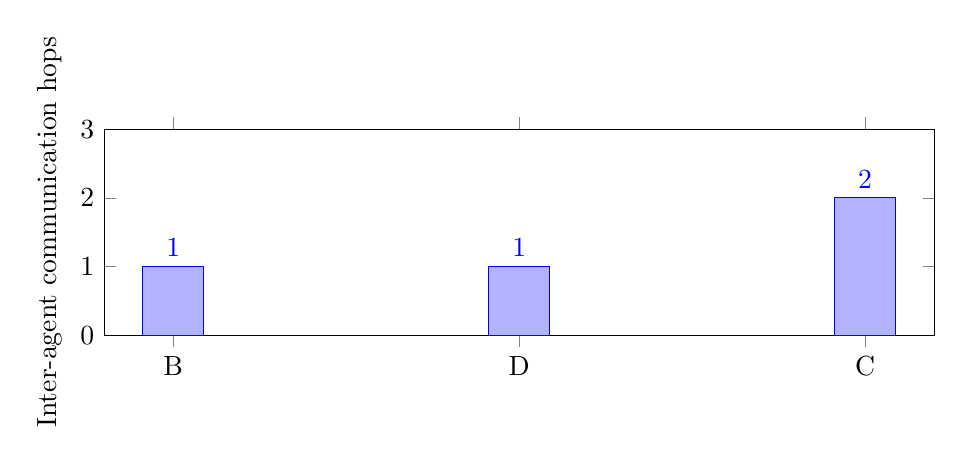
\begin{tikzpicture}
\begin{axis}[
  ybar, bar width=22pt, width=\linewidth, height=4.2cm,
  ylabel={Inter-agent communication hops},
  symbolic x coords={B,D,C}, xtick=data,
  ymin=0, ymax=3,
  nodes near coords,
]
\addplot coordinates {(B,1) (D,1) (C,2)};
\end{axis}
\end{tikzpicture}
\caption{Communication complexity across the experimental arms, measured by
the number of inter-agent communication hops. Arms B and D employ a
single-agent MCP workflow (1 hop), whereas Arm C introduces an additional A2A
interaction between the User Butler and Store Agent (2 hops).}
\label{fig:comm}
\end{figure}

\subsection{Security Evaluation}

\begin{figure}[t]
\centering
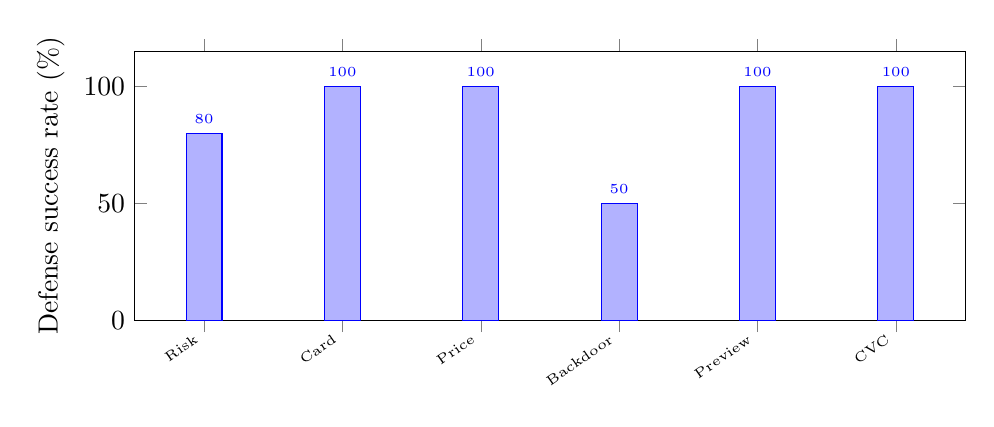
\begin{tikzpicture}
\begin{axis}[
  ybar, bar width=13pt, width=\linewidth, height=5.0cm,
  ylabel={Defense success rate (\%)},
  symbolic x coords={Risk,Card,Price,Backdoor,Preview,CVC},
  xtick=data, x tick label style={rotate=35, anchor=east, font=\tiny},
  ymin=0, ymax=115,
  nodes near coords, nodes near coords style={font=\tiny},
]
\addplot coordinates {(Risk,80) (Card,100) (Price,100) (Backdoor,50) (Preview,100) (CVC,100)};
\end{axis}
\end{tikzpicture}
\caption{Security regression evaluation across six attack categories (the
original four plus SEC-05/SEC-06 added in this revision). Purchase Risk:
8/10 (80\%, original baseline, exploratory, not re-run in this revision --
needs a live LLM call). Agent Card manipulation: 4/4 (100\%), independently
reproduced 2026-07-27. Price manipulation: 1/1 (100\%), independently
reproduced 2026-07-27. Backdoor attacks: 2/4 (50\%), independently reproduced
2026-07-27 -- the hardest category, since malicious intent can be hidden in
otherwise legitimate interactions. Preview tampering: 100\%, zero side
effects across all tampering attempts. CVC leakage: 100\%, the sentinel CVC
value never appeared in any request, response, or log artifact.}
\label{fig:security}
\end{figure}

Figure~\ref{fig:security} summarizes the security regression experiments
conducted on Arm C. The proposed architecture successfully defended against
manipulated Agent Cards and price manipulation attacks, achieving a 100\%
success rate in both categories. Purchase-risk attacks were correctly
handled in 80\% of the evaluated cases. Backdoor-style attacks remained the
most challenging scenario, with a 50\% defense success rate, indicating that
hidden intent manipulation remains an important direction for future
improvements. Although the backdoor evaluation remains preliminary, it
highlights the difficulty of defending against indirect semantic
manipulation. These results indicate that deterministic attacks can be
mitigated through policy validation, whereas semantic attacks remain
significantly more challenging because malicious intent may be hidden within
otherwise legitimate interactions.

The two categories added in this revision extend rather than soften that
conclusion: preview tampering and CVC leakage are both \emph{deterministic}
checks -- byte-equality against a server-owned preview, and substring
scanning for a sentinel value -- and both defended at 100\%, reinforcing that
mechanically checkable properties are exactly the ones bounded capability
exposure defends well, while semantic intent (backdoor attacks) is exactly
the ones it does not yet defend well.

Separately, the 15-scenario negative-path matrix (Table~\ref{tab:negpath})
was exercised against both the local deployment and the public Cloudflare
deployment (Sec.~\ref{sec:deploy}); the three scenarios repeated on both
(BUY-F01, missing field; BUY-F05, premature confirmation; BUY-F07, preview
mismatch) were rejected with zero purchase side effects on both deployments.

\subsection{Summary of Findings}

Overall, the experimental results reveal clear trade-offs among the evaluated
interoperability mechanisms. Direct GraphQL offers the highest efficiency,
whereas MCP and A2A improve interoperability, capability exposure, and trust
separation with additional communication overhead. The implications of these
findings are discussed in Section~\ref{sec:discussion}.

\section{Discussion}
\label{sec:discussion}

\subsection{Answering the Research Questions}

This study investigated how MiSArch capabilities can be exposed to
autonomous agents through different interoperability mechanisms and what
trade-offs these interfaces introduce. The results indicate that no single
interface is optimal for all scenarios. Instead, each architecture provides
different benefits depending on the deployment objective.

Regarding RQ1, direct GraphQL remains the most efficient interface for
backend services, while MCP introduces additional latency and communication
overhead. However, MCP also provides structured tool discovery, typed
schemas, provenance information, and explicit side-effect descriptions,
making backend capabilities easier for autonomous agents to understand and
invoke~\cite{ref2,ref3,ref9}. Therefore, protocol standardization becomes
worthwhile when interoperability, maintainability, and safe capability
exposure are more important than minimizing latency.

For RQ2, our experiments demonstrate that metadata improves discoverability
but should not be considered trustworthy by default. Although malicious
Agent Cards and manipulated prices were successfully detected, some hidden
purchase intents still bypassed the current safety mechanism. This suggests
that metadata should support capability discovery, but all security-critical
decisions must rely on independent validation rather than advertised
descriptions~\cite{ref5,ref6}. The preview-tampering and CVC-leakage
regressions added in this revision (100\% each) show the mechanism scales to
new deterministic properties for free once the pattern -- validate against a
server-owned value, never trust the client's restated value -- is in place.

Finally, RQ3 highlights that trust boundaries should remain under local
control. MCP tool schemas and A2A Agent Cards improve interoperability, but
they should not become security boundaries themselves. Instead, authorization,
policy enforcement, and confirmation mechanisms should remain within trusted
local components such as the gateway or user butler~\cite{ref3,ref5}. The
public Cloudflare deployment (Sec.~\ref{sec:deploy}) demonstrates this same
principle holds once the trust boundary is also a real network boundary: the
confirmation gate and preview-matching logic run entirely on the store-agent
side and required no change to work over public HTTPS.

\subsection{Trade-offs of Different Agent Interfaces}

The evaluation shows that the four architectures represent different design
trade-offs rather than a performance ranking. Direct GraphQL provides the
lowest latency and is well suited for internal backend communication. MCP
introduces moderate protocol overhead but significantly improves
discoverability, structured tool invocation, and traceability~\cite{ref2,ref9}.
A2A further extends the architecture by separating user and merchant trust
domains, allowing user preferences to remain local while enabling cross-agent
collaboration~\cite{ref3}.

Consequently, interface selection should depend on deployment requirements.
Low-risk internal services benefit from the efficiency of GraphQL, whereas
agent-facing requires additional structure and bounded capability exposure
through MCP or A2A despite the extra communication cost.

These architectures therefore complement rather than replace one another.
Internal cloud-native services may prioritize efficiency through GraphQL,
whereas agent ecosystems involving heterogeneous organizations benefit from
standardized capability exposure through MCP and explicit trust separation
through A2A.

\subsection{Discoverability and Self-Describing Interfaces}

One of the key differences between direct GraphQL and MCP lies in capability
discoverability. Direct GraphQL provides flexible backend access but assumes
that clients already understand the available schema and construct valid
queries. In contrast, MCP exposes a curated set of tools with explicit
descriptions, structured input schemas, and side-effect metadata, allowing
autonomous agents to reason about available capabilities before execution.

A2A extends this idea through Agent Cards, which advertise the capabilities
of remote agents. However, unlike local MCP tools, Agent Cards cross trust
boundaries and therefore support discoverability rather than authorization.
Consequently, discoverability should be complemented by local validation and
policy enforcement rather than relying solely on advertised metadata.

\subsection{Side-Effect Control}

Not all backend capabilities should be exposed equally to external agents.
Read-only operations, such as product browsing, involve little risk and can
be safely exposed through standardized interfaces. In contrast,
state-changing operations, including pending order creation or payment
execution, require stronger validation, confirmation, and policy
enforcement.

The security evaluation demonstrates that safe capability exposure depends
not only on protocol design but also on restricting which operations are
externally accessible. Therefore, capability selection should consider both
operational risk and reversibility rather than exposing all backend APIs
uniformly. The negative-path matrix in Table~\ref{tab:negpath} operationalizes
this principle for the purchase skill specifically: every one of its 15
failure categories is required to produce zero \emph{new} purchase side
effects, which is a stronger and more testable claim than ``requires
confirmation'' alone.

\subsection{Security Implications}

The security evaluation demonstrates that interoperability protocols
introduce new attack surfaces beyond traditional APIs. Tool descriptions, MCP
schemas, and Agent Cards facilitate agent cooperation but may also contain
misleading or malicious information~\cite{ref2,ref6}. Our experiments show
that deterministic policy checks successfully defended against manipulated
Agent Cards, fake prices, tampered previews, and CVC exfiltration attempts,
whereas semantic attacks such as hidden purchase intent remained more
difficult to detect.

These findings suggest that metadata should only be used for capability
discovery. Sensitive operations should always be protected through local
policy enforcement, explicit confirmation, and independent validation rather
than relying on externally advertised metadata.

\subsection{Practical Implications}

For MiSArch, the results support a layered deployment strategy. GraphQL
should remain the internal data interface because of its flexibility and
efficiency~\cite{ref9}. MCP is appropriate for exposing selected backend
capabilities as standardized tools for external agents~\cite{ref2}, while A2A
is more suitable when communication crosses organizational or trust
boundaries~\cite{ref3}.

Overall, our findings suggest that future cloud-native agent systems should
prioritize bounded capability exposure, explicit trust separation, and
auditable interfaces rather than optimizing for latency alone.

\section{Limitations and Future Work}
\label{sec:limitations}

This study has several limitations that should be considered when
interpreting the results. First, the current MiSArch catalog contains only a
limited number of products, which restricted the evaluation of personalized
recommendation and complete purchase workflows -- this limitation is
unchanged from the original evaluation. Second, the A2A prototype is no
longer as simplified as originally reported: it now runs the official
\texttt{a2asrv} task lifecycle end to end (submit $\rightarrow$
input-required $\rightarrow$ completed/failed) and closes the purchase loop
to a real \texttt{PLACED}/\texttt{SUCCEEDED} outcome (Sec.~\ref{sec:purchase}),
including over a public network boundary (Sec.~\ref{sec:deploy}); it remains
a research prototype without streaming, push notifications, durable task
storage, signed Agent Cards, or production A2A authentication. Third,
although the security evaluation now covers six representative adversarial
scenarios instead of four, the number of trials per category remains small
and cannot fully characterize the robustness of the proposed architectures;
Purchase-Risk regression in particular was not independently re-executed in
this revision because it requires a live LLM call.

This revision also surfaces one concrete, previously unreported limitation:
\texttt{CompletePurchase}'s payment-attribution step
(\texttt{waitForPayment} in \texttt{internal/order/service.go}) identifies
``the'' new payment for a purchase by diffing the set of payment IDs before
and after placing the order, filtered only by \texttt{payment\_information\_id}.
Two concurrent purchases sharing the same payment method are not
distinguished by this diff, so under concurrency the wrong payment could in
principle be attributed to the wrong task (BUY-F15 in
Table~\ref{tab:negpath}). This is discussed further as a code-level finding
in the accompanying engineering review and is tracked as future work rather
than fixed in this revision.

Future work should therefore extend the MiSArch catalog with richer product
data, improve intent detection for indirect purchase requests, and evaluate
more realistic malicious-agent behaviors, in particular re-running the
Purchase-Risk regression against the current code with a live model in the
loop. In addition, stronger authentication, prompt-injection defenses, formal
privacy verification, and a concurrency-safe payment-attribution mechanism
should be incorporated to better assess trust propagation and profile
protection in agent interoperability systems~\cite{ref5,ref6}. Expanding the
benchmark with more tasks and larger-scale experiments would also provide
stronger evidence for the architectural trade-offs identified in this
work~\cite{ref7}.

Future work will also investigate larger-scale cloud deployments involving
multiple organizations, dynamic service discovery, and heterogeneous agent
ecosystems, building on the Cloudflare deployment already validated in
Sec.~\ref{sec:deploy} by moving from a Worker Free tier tunneled to a
developer machine to an independently-durable Container deployment.
Evaluating interoperability under real production workloads would provide
stronger evidence for the practical applicability of the proposed
architecture.

\section{Conclusion}

This work presented a comparative study of four interoperability mechanisms
for exposing MiSArch capabilities to autonomous agents. The evaluation
demonstrated that GraphQL provides the highest efficiency for backend
communication, whereas MCP improves interoperability through standardized
tool descriptions and structured capability exposure~\cite{ref2,ref9}.
Furthermore, A2A extends the architecture by enabling collaboration across
trust domains while maintaining stronger separation of user profiles and
merchant services~\cite{ref3}.

Our security experiments further showed that protocol metadata improves
capability discovery but should not be relied upon as a security boundary.
Instead, authorization and policy enforcement should remain under local
control to defend against prompt injection, tool poisoning, and malicious
metadata~\cite{ref5,ref6}.

Relative to the original study, this revision demonstrates that the same
architecture, once its purchase skill is driven to a real completed order
and payment and deployed across a public network boundary, preserves every
one of the original trade-off conclusions while adding two new deterministic
security guarantees (preview tampering, CVC leakage) essentially for free.
The one new gap this revision surfaces -- payment attribution under
concurrent purchases -- is a code-level concurrency issue, not an
architectural one, and is scoped as future work.

The results suggest that the choice of interoperability mechanism should be
guided by deployment requirements rather than performance alone. Future
cloud-native agent systems will benefit from architectures that balance
efficiency, interoperability, and trustworthy capability exposure. These
findings provide practical guidance for designing future cloud-native AI
systems that balance efficiency, interoperability, and trustworthy capability
exposure.

Overall, the main conclusion is that agent interoperability should not be
evaluated only by raw performance or connectivity. For external AI agents,
the more important question is whether the system exposes the right
capabilities through the right boundary.

\begin{thebibliography}{9}

\bibitem{ref1}
L. Wang, C. Ma, X. Feng, Z. Zhang, H. Yang, J. Zhang, Z. Chen, J. Tang, X.
Chen, Y. Lin, W. X. Zhao, Z. Wei, and J.-R. Wen, ``A survey on large language
model based autonomous agents,'' \emph{Frontiers of Computer Science}, 2024,
arXiv:2308.11432. [Online]. Available: \url{https://arxiv.org/abs/2308.11432}

\bibitem{ref2}
A. Ehtesham, A. Singh, G. K. Gupta, and S. Kumar, ``A survey of agent
interoperability protocols: Model context protocol (mcp), agent
communication protocol (acp), agent-to-agent protocol (a2a), and agent
network protocol (anp),'' 2025. [Online]. Available:
\url{https://arxiv.org/abs/2505.02279}

\bibitem{ref3}
C. Jeong, ``A study on the mcp $\times$ a2a framework for enhancing
interoperability of llm-based autonomous agents,'' 2025. [Online]. Available:
\url{https://arxiv.org/abs/2506.01804}

\bibitem{ref4}
Y. Liu, S. K. Lo, Q. Lu, L. Zhu, D. Zhao, X. Xu, S. Harrer, and J. Whittle,
``Agent design pattern catalogue: A collection of architectural patterns for
foundation model based agents,'' \emph{Journal of Systems and Software}, vol.
220, p. 112278, 2025. [Online]. Available:
\url{https://doi.org/10.1016/j.jss.2024.112278}

\bibitem{ref5}
N. Maloyan and D. Namiot, ``Breaking the protocol: Security analysis of the
model context protocol specification and prompt injection vulnerabilities in
tool-integrated llm agents,'' 2026. [Online]. Available:
\url{https://arxiv.org/abs/2601.17549}

\bibitem{ref6}
C. Huang, X. Huang, N. P. Tran, and A. M. Fard, ``Model context protocol
threat modeling and analyzing vulnerabilities to prompt poisoning with tool
poisoning,'' 2026. [Online]. Available: \url{https://arxiv.org/abs/2603.22489}

\bibitem{ref7}
Z. Wang, Q. Chang, H. Patel, S. Biju, C.-E. Wu, Q. Liu, A. Ding, A.
Rezazadeh, A. Shah, Y. Bao, and E. Siow, ``Mcp-bench: Benchmarking
tool-using llm agents with complex real-world tasks via mcp servers,'' 2025.
[Online]. Available: \url{https://arxiv.org/abs/2508.20453}

\bibitem{ref8}
S. Yao, J. Zhao, D. Yu, N. Du, I. Shafran, K. Narasimhan, and Y. Cao,
``React: Synergizing reasoning and acting in language models,'' in
\emph{International Conference on Learning Representations (ICLR)}, 2023,
arXiv:2210.03629. [Online]. Available: \url{https://arxiv.org/abs/2210.03629}

\bibitem{ref9}
E. Wittern, A. Cha, J. C. Davis, and L. Mandel, ``An empirical study of
graphql design patterns,'' in \emph{Service-Oriented Computing (ICSOC 2019)}.
Springer, 2019, pp. 3--19. [Online]. Available:
\url{https://doi.org/10.1007/978-3-030-33702-5_1}

\end{thebibliography}

\end{document}
